\chapter{觀測、暗物質與宇宙學擬合}

\lectureoverview{觀測只有和宇宙學模型連結起來，才有意義。我們從弗里德曼方程和三種均勻空間幾何出發，將當今的宇宙能量預算整理為輻射、物質、真空能與曲率，並重建開放宇宙為何一度被視為無可避免。接著，星系旋轉曲線揭示了缺失的引力物質，並引出冷、弱交互作用暗暈的動力學。最後，紅移、亮度和源計數將試探性的膨脹歷史轉化為可觀測曲線。舊的物質加曲率模型無法符合觀測；物質分率約為\(0.3\)、真空分率約為\(0.7\)且曲率極小，則得到本講的成功擬合。}

\section{將觀測帶回方程}

天文觀測事實不能孤立解讀。我們首先需要方程，才能知道哪些觀測量的組合可以區分不同的宇宙。對均勻且各向同性的宇宙，出發點是弗里德曼方程，
\begin{equation}
\left(\frac{\dot a}{a}\right)^2
=
\frac{8\pi G}{3}\rho-\frac{k}{a^2}.
\label{eq:c06-friedmann}
\end{equation}
其中的量
\begin{equation}
H(t)=\frac{\dot a(t)}{a(t)}
\label{eq:c06-hubble}
\end{equation}
是哈伯\emph{函數}。它在當下的值\(H_0\)慣稱哈伯常數，但\(H(t)\)並非在整個宇宙歷史中都保持不變。天文學家以每秒每百萬秒差距幾公里的單位報出數值時，指的就是\(H_0\)。

歸一化曲率標記只可能取三個值，
\begin{equation}
k\in\{+1,0,-1\},
\end{equation}
分別對應球面、平坦與雙曲空間幾何。常用的 FRW 度規可寫成
\begin{equation}
ds^2=-dt^2+a(t)^2\left[dr^2+\xi(r)^2d\Omega_2^2\right],
\label{eq:c06-frw}
\end{equation}
其中
\begin{equation}
\xi(r)=
\begin{cases}
\sin r, & k=+1,\\
r, & k=0,\\
\sinh r, & k=-1.
\end{cases}
\label{eq:c06-xi}
\end{equation}
這個記號有兩個用途：它將三種幾何整合在同一個度規中，之後也會給出球面的面積，從而決定徑向殼層中的源數量。因此，選定\(k\)並給出\(a(t)\)的方程，就已經構成一個具有可觀測後果的模型。

\section{當今的宇宙能量預算}

在這裡討論的模型中，能量密度有三個主要成分：輻射、非相對論性物質和真空能。將曲率也列入同一個帳目，可得
\begin{equation}
\frac{C_r}{a^4}
+\frac{C_m}{a^3}
+\Lambda
-\frac{k}{a^2}
=H^2.
\label{eq:c06-budget}
\end{equation}
此處\(\Lambda\)採用上一講的歸一化方式，\(\Lambda=(8\pi G/3)\rho_{\rm vac}\)。輻射密度隨\(a^{-4}\)遞減，物質密度隨\(a^{-3}\)遞減，真空能不會稀釋，而曲率項則依\(a^{-2}\)縮放。曲率不是物質的能量密度，但將它與其他項並列，就能清楚看出當下的約束：四項貢獻的總和必須等於\(H_0^2\)。

將它們當下的分率定義為
\begin{equation}
\begin{aligned}
\Omega_r&=\frac{C_r/a_0^4}{H_0^2},
&\qquad
\Omega_m&=\frac{C_m/a_0^3}{H_0^2},\\
\Omega_\Lambda&=\frac{\Lambda}{H_0^2},
&
\Omega_k&=\frac{-k/a_0^2}{H_0^2}.
\end{aligned}
\label{eq:c06-omegas}
\end{equation}
於是
\begin{equation}
\boxed{\Omega_r+\Omega_m+\Omega_\Lambda+\Omega_k=1.}
\label{eq:c06-sum-rule}
\end{equation}
這些\(\Omega\)是以今日的數值計算出的比率，並非不隨時間改變的常數。也請留意符號慣例：\(k=-1\)會給出正的\(\Omega_k\)。

\subsection{如何測量最初幾項}

哈伯藉由比較退行紅移與距離，測得局部的膨脹率。在低\(z\)時，紅移可給出速度；經過校準的亮度則可給出距離。他最初得到的數值錯得很離譜，但方法是正確的。由於那些星系相對較近，測量並未涵蓋宇宙歷史中很長的一段，因此可以將\(H\)視為當下的值。

\begin{classroomqa}
\audiencequestion{若不知道天體的內禀亮度，怎麼能用亮度測出距離？}
\lecturerresponse{無法一步做到。宇宙距離階梯從近距離恆星的視差測量開始。經過校準的鄰近區域中，造父變星呈現出週期－光度關係，因此可作為較遠距離的標準燭光。透過彼此重疊的校準逐步延伸距離階梯，而超新星則是在後續所用宇宙學紅移範圍內最好的標準燭光。因此，距離是由一連串標準推斷而得，並非任意假設每個天體的發光程度都相同。 \lecturetimestamp{00:10:00--00:11:32}}
\end{classroomqa}

\begin{classroomqa}
\audiencequestion{即使\(C_r\)和\(C_m\)的密度會改變，它們仍是常數嗎？}
\lecturerresponse{是的。係數保持固定，而\(a^{-4}\)和\(a^{-3}\)這些因子則帶有時間依賴性。真空能是常數，曲率則依\(a^{-2}\)縮放。正是這些不同的冪次，使各分率的貢獻隨時代而變化。 \lecturetimestamp{00:11:35--00:12:02}}
\end{classroomqa}

輻射項可透過局部的光子背景測量，其中大部分是宇宙微波背景。相較於其他重要成分，輻射在當下的能量密度極小。測量需要足夠大的平均體積，但不必沿著過去光錐回溯很遠，就能確認\(\Omega_r\)今日可忽略不計。

可見物質的含量可由星系、恆星族群、氫和星際氣體估算。這些方法在技術上較繁複，但概念並不晦澀：先確定典型的恆星與氣體含量，再對星系加總，最後在大體積範圍內取平均。本講引用過去的粗略估計：每立方公尺約有一個質子的質量。這比輻射密度大得多，但仍稀薄得驚人。

\begin{classroomqa}
\audiencequestion{那麼，這份帳目中的暗物質呢？}
\lecturerresponse{接下來就會談到；不過我們先刻意重建僅根據發光物質所作的舊推論。這段歷史脈絡很重要，因為它清楚指出暗物質修正了哪個表面上的結論，又沒有填補哪個缺口。 \lecturetimestamp{00:15:08--00:15:40}}
\end{classroomqa}

\section{開放宇宙為何一度被視為必要}

在較早的圖像中，輻射被正確判定為可忽略，真空能設為零，而物質只包括能透過電磁輻射觀測到的物質。由此得到的估計約為
\begin{equation}
\Omega_r\simeq0,
\qquad
\Omega_\Lambda=0,
\qquad
\Omega_m^{\rm luminous}\sim\frac{1}{20}\text{--}\frac{1}{30}.
\end{equation}
於是，求和規則似乎要求
\begin{equation}
\Omega_k\simeq1.
\end{equation}
由於正的曲率貢獻代表\(-k/a_0^2>0\)，這便意味著\(k=-1\)：宇宙是開放且具有負曲率。這些數值是對舊論證的重建，並非現代的參數估計。

為了解讀曲率尺度，回到物質主導時期的解
\begin{equation}
a(t)\propto t^{2/3}.
\end{equation}
對它微分並除以\(a\)，得到
\begin{equation}
H(t)=\frac{\dot a}{a}=\frac{2}{3t}.
\label{eq:c06-matter-h}
\end{equation}
在宇宙當前年齡\(T\)時，
\begin{equation}
H_0\simeq\frac{2}{3T}.
\end{equation}
因此，哈伯時間與宇宙年齡大致同量級。與輻射主導時期的情況比較，
\begin{equation}
a(t)\propto t^{1/2},
\qquad
H(t)=\frac{1}{2t},
\end{equation}
可知這種年齡倒數關係並非塵埃物質所獨有。

\begin{figure}[htbp]
\centering
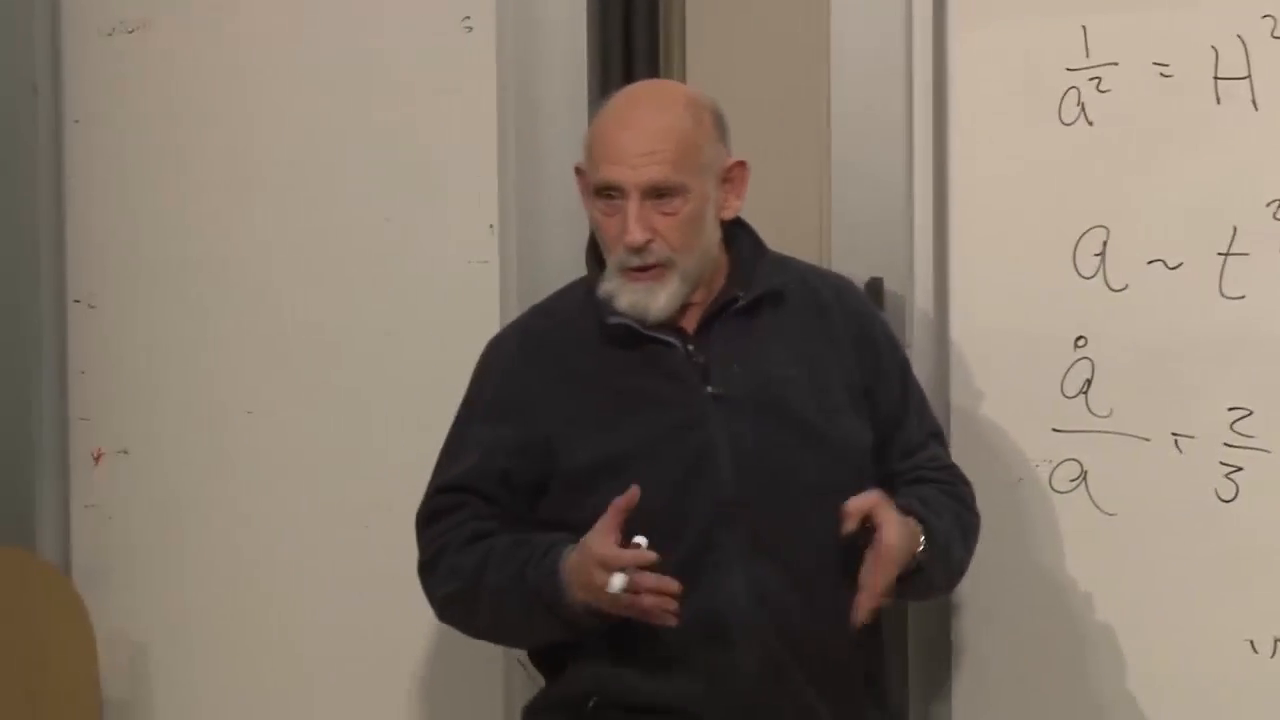
\includegraphics[width=0.72\textwidth]{lecture_06_figure_02.png}
\caption{物質主導時期的板書回顧。畫面上可見\(a\sim t^{2/3}\)和\(\dot a/a=2/(3t)\)；講師遮住黑板其餘部分，因此不將任何看不見的方程歸於這個畫面。}
\label{fig:c06-age-board}
\lectureframe{00:24:41.615}
\end{figure}

\begin{classroomqa}
\audiencequestion{哈伯常數的單位是什麼？光速又在哪裡？}
\lecturerresponse{由於\(H\)表示速度與距離的比值，它的單位是時間的倒數。可以用每秒的倒數、每年的倒數，或天文學家慣用的等價單位「每秒每百萬秒差距幾公里」表示。關係式\(H\sim1/T\)不需要額外乘上\(c\)。只有在將時間\(c\)換算成像\(T\)這樣的長度時，才會出現\(cT\)因子。\lecturetimestamp{00:22:50--00:24:25}}
\end{classroomqa}

哈伯最初測得的\(H_0\)大約大了一個數量級，因此相應的哈伯年齡太短；依本講取整後的比較，大約是十億年，而非一百億年。更精確的校準修正了數值，但沒有改變\(H_0^{-1}\)代表宇宙時間尺度這個道理。

舊有的曲率推論可寫成
\begin{equation}
\frac{1}{a_0^2}\sim H_0^2\sim\frac{1}{T^2}.
\end{equation}
在\(c=1\)單位制下，曲率半徑\(a_0\)因此被認為與宇宙年齡\(T\)同量級；換回一般單位後，則約為\(cT\)。本講隨即撤回這項說法，並不將它視為真實宇宙的描述。這是幾十年前捨棄當時被認為可忽略的項之後所得出的結論。

\begin{classroomqa}
\audiencequestion{如果曲率被認為今天應該占主導地位，為什麼還使用物質主導定律\(a\propto t^{2/3}\)？}
\lecturerresponse{因為物質項隨\(a^{-3}\)縮放，而曲率項只隨\(a^{-2}\)縮放。在較小的\(a\)時，物質項占優勢。曲率只有到了晚期才可能變得重要，因此物質主導仍描述了大部分已經過去的歷史，也使\(H_0\)維持在\(1/T\)的量級。完整的混合解會修正數值因子，但不會推翻這個時間尺度論證。 \lecturetimestamp{00:49:20--00:50:17}}
\end{classroomqa}

\section{從星系動力學看見暗物質}

清查物質有兩種實際方法：一種是計算會發射或吸收光的物質，另一種是從引力推斷質量。奧爾特在1930年代初發現星系動力學的異常，茲威基則在星系團中發現類似的質量差異。證據顯示，引力所反映的物質多於發光物質。普通帶電物質會輻射並發生碰撞；這種缺失成分最初是透過其引力效應被發現的。

\begin{classroomqa}
\audiencequestion{發光物質包括稀薄氣體和中心黑洞嗎？}
\lecturerresponse{只要能根據電磁效應推斷稀薄氣體的含量，就會將它計入。中心超大質量黑洞可能也會列入已知質量的帳目，但它只占星系總質量的一小部分，而且集中在中心。它無法解釋在發光中心以外很遠仍然存在的質量差異。 \lecturetimestamp{00:29:50--00:31:14}}
\end{classroomqa}

考慮一顆大致沿半徑為\(r\)的圓軌道運行的恆星。如果幾乎全部質量\(M\)都集中在星系中心附近，牛頓定律會給出
\begin{equation}
\frac{GM}{r^2}=\frac{v^2}{r},
\end{equation}
因此
\begin{equation}
v^2=\frac{GM}{r},
\qquad
v(r)\propto r^{-1/2}.
\label{eq:c06-kepler}
\end{equation}
這就是中心質量分布之外預期的開普勒式衰減。

\begin{figure}[htbp]
\centering
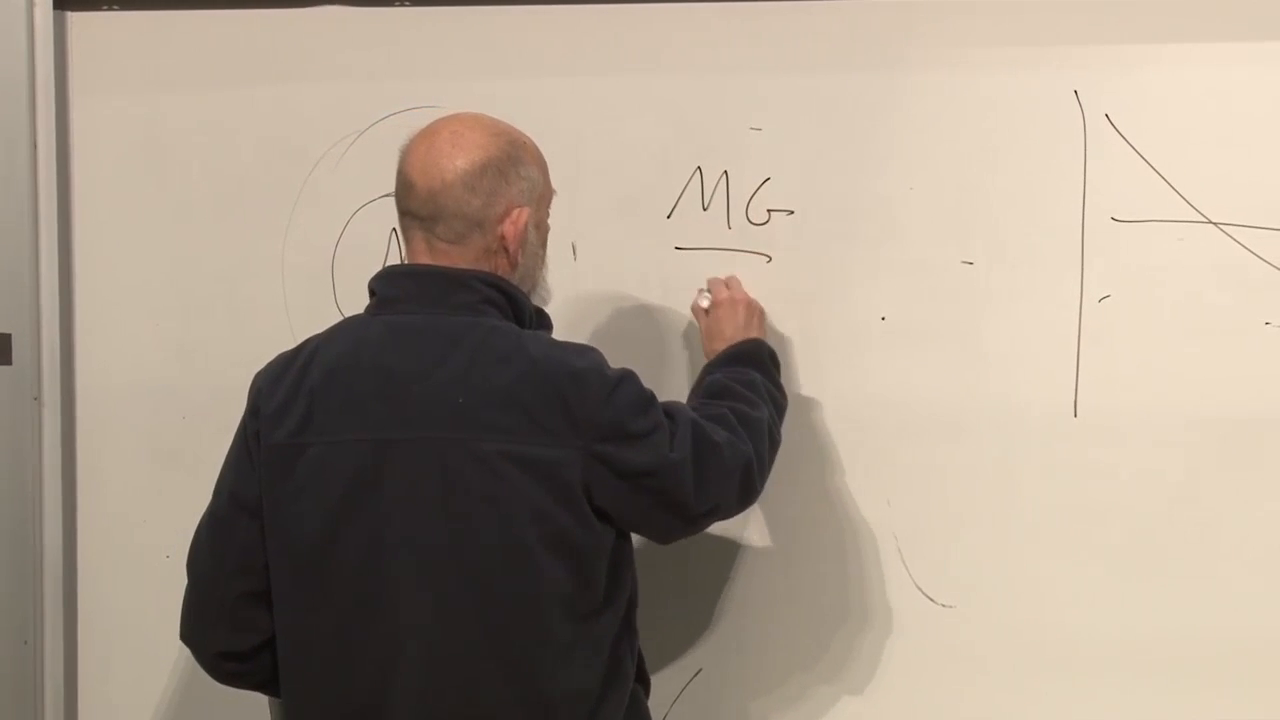
\includegraphics[width=0.78\textwidth]{lecture_06_figure_03.png}
\caption{旋轉曲線板書：從中心質量轉換為半徑內的總質量\(M(r)\)。畫面只看得到\(MG\)、分數線、軌道草圖及部分曲線草圖；方程~\eqref{eq:c06-kepler}則來自口頭推導。}
\label{fig:c06-rotation-board}
\lectureframe{00:34:53.642}
\end{figure}

\begin{figure}[htbp]
\centering
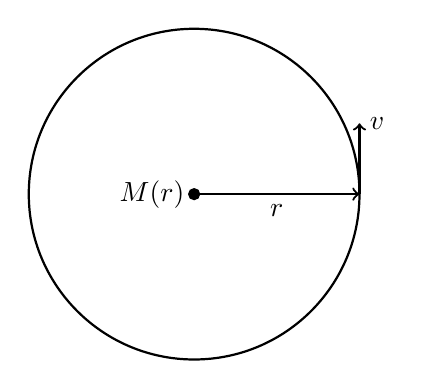
\begin{tikzpicture}[scale=1.0]
\filldraw (0,0) circle (2pt) node[left] {\(M(r)\)};
\draw[thick] (0,0) circle (2.1);
\draw[->,thick] (0,0)--(2.1,0) node[midway,below] {\(r\)};
\draw[->,thick] (2.1,0)--(2.1,0.9) node[right] {\(v\)};
\end{tikzpicture}
\caption{利用圓軌道構造，從測得的旋轉速度推算半徑內的總質量。}
\label{fig:c06-orbit-redraw}
\end{figure}

觀測到的星系旋轉曲線並未如此下降；在相當大的半徑範圍內，曲線大致平坦。將固定的中心質量改為半徑內的總質量\(M(r)\)：
\begin{equation}
\frac{G M(r)}{r^2}=\frac{v(r)^2}{r}.
\end{equation}
若\(v(r)\)大致維持不變，則
\begin{equation}
\boxed{M(r)\propto r.}
\label{eq:c06-enclosed-mass}
\end{equation}
這裡指的是半徑\(r\)以內的總質量，而非局部密度。引力所反映的總質量在大部分星光集中的區域以外，仍持續增加。垂直於星系盤面的運動進一步指出，物質大致呈球形分布：也就是暗暈，而非另一個薄盤。

\begin{classroomqa}
\audiencequestion{有沒有簡單的理論能解釋旋轉曲線為何如此平坦？}
\lecturerresponse{這段論證沒有提供這樣的理論。星系形成模擬或許能讓這類分布顯得自然，但本講並未聲稱能簡單推導出來。可靠的觀測結論是：\(v\)大致恆定，代表半徑內的總質量大致隨半徑線性增加。這個關係雖然簡潔，卻不應被誤認為星系形成的簡單解釋。 \lecturetimestamp{00:35:58--00:37:33}}
\end{classroomqa}

\begin{classroomqa}
\audiencequestion{旋臂只是角速度\(v/r\)變化所形成的物質風車嗎？}
\lecturerresponse{簡單的風車圖像並不成立。可見的圖樣不一定和個別恆星一起旋轉；密度波或恆星形成波都是可能的描述。本講藉此不確定性，區分穩健的暗暈推論與更複雜的旋臂結構問題。 \lecturetimestamp{00:37:35--00:38:34; 00:47:03--00:47:47}}
\end{classroomqa}

推論出的暗物質質量是發光物質的數倍；本講只將其粗略估為約五至十倍。暗暈也延伸至可見星系之外。這些是刻意給出的粗略歷史尺度，並非適用於每個星系的精確普遍比值。

\section{暗物質必須具備哪些性質}

為什麼普通物質會形成明亮、緻密的盤，而暗物質卻分布在廣大的暈中？發光物質能藉由電磁碰撞和輻射失去機械能。能量耗散後，引力便能將它拉入更緻密的構型。暗物質似乎不帶電，且交互作用微弱得多。暗物質粒子在暈中運行時，幾乎不發生碰撞或輻射，因此即使經過數十億年，也不會失去足夠能量而沉降至發光物質形成的盤中。星系運動產生的重力輻射弱得多，無法提供另一種冷卻機制。

\begin{classroomqa}
\audiencequestion{弱交互作用是否表示暗物質遵循不同的引力定律？}
\lecturerresponse{不是。假設暗物質以一般方式受引力作用。此處所說的弱交互作用，是指非引力碰撞和電磁輻射不存在或受到大幅抑制。兩個暗物質粒子仍會透過引力相互吸引；這種吸引能形成暗暈，卻無法有效耗散軌道能量。 \lecturetimestamp{00:42:36--00:43:35}}
\end{classroomqa}

\begin{classroomqa}
\audiencequestion{有哪些觀測顯示，這並非單一星系旋轉曲線的特殊現象？}
\lecturerresponse{證據涵蓋多種尺度：星系內恆星的運動、垂直於星系平面的運動、星系之間的交互作用，以及整個星系團的動力學。奧爾特和茲威基的例子，是同一個缺失引力問題在不同尺度上的表現。 \lecturetimestamp{00:42:00--00:42:36}}
\end{classroomqa}

\begin{classroomqa}
\audiencequestion{暗物質應該聚集在黑洞和星系中心周圍嗎？}
\lecturerresponse{暗物質確實會在引力中心附近變得較密集，但歷史發展的順序很可能不是暗暈圍繞著早已存在的黑洞形成。暗暈先形成巨大的引力勢阱；接著重子物質落入其中，形成星系、恆星和中心黑洞。黑洞只占總質量的一小部分。儘管如此，搜尋湮滅產物時仍會觀測星系中心，因為預期那裡的暗物質密度較高。 \lecturetimestamp{00:43:36--00:45:43}}
\end{classroomqa}

\begin{classroomqa}
\audiencequestion{暗物質是氣體、塵埃、緻密團塊，還是分散的粒子？有些暗物質會被束縛在太陽附近嗎？}
\lecturerresponse{暗物質的微觀本質尚不清楚，但普通塵埃受電磁力束縛，而暗物質似乎恰好缺乏這類交互作用。因此，預設的粒子圖像是一群稀疏分布的個別粒子。有些粒子可能受引力聚集在太陽附近，但密度遠低到不足以和太陽引力抗衡，也不會擾亂行星動力學。 \lecturetimestamp{00:45:43--00:47:02; 00:58:41--00:59:29}}
\end{classroomqa}

第二個關鍵要求是暗物質必須能聚集。具有相對論性隨機速度的熱粒子族群會抗拒引力聚集；冷粒子族群則能落入勢阱。普通的輕中微子會成為熱暗物質，無法構成所需的星系主要成分。在此脈絡下，\emph{冷}是指在局部宇宙學參考系中屬於非相對論性，而非字面上的實驗室零溫。

\begin{classroomqa}
\audiencequestion{冷暗物質能聚集的要求，是否限制了暗物質的質量範圍？}
\lecturerresponse{這取決於量子統計和產生歷史。極輕的費米子無法全都占據同一個低速態，因此受到嚴格限制。極輕的玻色子則能占據相干的玻色－愛因斯坦凝聚態；軸子就是本講舉的例子。另一種可能是較重的弱交互作用粒子，無需凝聚也能成為冷暗物質。因此，這個論證無法給出一個不依賴模型的單一質量界限。 \lecturetimestamp{00:53:17--00:54:52; 00:56:42--00:58:05}}
\end{classroomqa}

\begin{classroomqa}
\audiencequestion{加速器不是早就應該發現這些粒子了嗎？}
\lecturerresponse{只有在額外假設成立時才是如此。如果這些粒子的交互作用截面大致相當於弱交互作用，且質量落在加速器可探測的範圍內，對撞機就可能產生它們。本講對近期即可取得相關資訊的預期，明確屬於推測，也帶有特定的歷史背景。粒子也可能太重，或交互作用太微弱，以致現有實驗無法探測。 \lecturetimestamp{00:54:52--00:55:54}}
\end{classroomqa}

\begin{classroomqa}
\audiencequestion{暗物質會不會只是存在於看不見的額外維度中？}
\lecturerresponse{這段討論不需要這種機制。暗物質已透過引力效應被觀測到；它或許只是由幾乎不與普通物質交互作用的特殊粒子構成。將交互作用稱為「弱」，並不表示這些粒子位於可觀測時空之外。 \lecturetimestamp{00:55:54--00:56:41}}
\end{classroomqa}

以修改引力取代增加不可見物質，是合乎邏輯的另一種可能。本講認為，當時沒有同樣簡單的引力修正，能在保留成功的太陽系定律之餘，同時解釋所有相關尺度上的證據。因此，較傾向採用粒子解釋，但暗物質的微觀物理仍然未知。

\section{暗物質仍無法補足舊的宇宙預算}

暗物質會使物質貢獻增加數倍，但舊估計中，發光物質與\(H_0^2\)之間的差距約為二十五倍。因此，暗物質雖縮小了差距，仍不足以使
\begin{equation}
\frac{C_m}{a_0^3}=H_0^2.
\end{equation}
成立。在舊的、不含\(\Lambda\)的圖像中，仍需要一個正的曲率預算項，也就是\(k<0\)。這類開放模型在邏輯上並無矛盾；重點是，單靠暗物質仍無法得到現代的答案。

\begin{classroomqa}
\audiencequestion{現代擬合出現之前，宇宙學家對曲率的實際看法是什麼？}
\lecturerresponse{當時的證據令人困惑，而偏好封閉、有界宇宙的想法，有時會與物質預算相牴觸。將舊有假設一致地結合後，負曲率便是自然的推論。這項歷史共識仍屬暫定，因為當時尚未像今日這樣確切納入暗物質和真空能。 \lecturetimestamp{00:50:17--00:51:50}}
\end{classroomqa}

因此，我們必須檢驗候選模型，而不能只根據一項預算推斷它是否正確。模型由曲率的選擇\(k\)和膨脹歷史\(a(t)\)構成；等價地說，它包含一組物質的狀態方程和當下參數，據此計算出\(a(t)\)。舊的候選模型只有物質和負曲率，輻射可忽略，也不含宇宙學常數。

\section{將幾何轉化為可觀測量}

\subsection{固定幾何中的源計數與亮度}

暫時忽略宇宙演化。在均勻宇宙中，共動殼層內的源數量正比於其面積：
\begin{equation}
dN\propto \xi(r)^2\,dr.
\label{eq:c06-shell-count}
\end{equation}
因此
\begin{equation}
dN\propto
\begin{cases}
\sin^2r\,dr, & k=+1,\\
r^2\,dr, & k=0,\\
\sinh^2r\,dr, & k=-1.
\end{cases}
\end{equation}
當\(r\)很大時，負曲率情形會依\(\sinh^2r\sim e^{2r}\)增長，遠快於平坦情形的\(r^2\)律。因此，負曲率預測源數量會隨距離異常快速增加。

同樣的面積也決定接收到的通量。在平坦的靜態空間中，標準光源給出
\begin{equation}
F\propto\frac{1}{r^2}.
\end{equation}
在雙曲空間中，輻射散布所經過的球面面積增長得更快，因此通量下降也更快。本講有時將這個觀測量稱為光度；此處\(F\)表示亮度或通量，內禀光度則是光源本身的性質。因此，結合源計數與亮度便能區分不同的空間幾何。

\subsection{紅移與過去光錐}

真實宇宙會演化，向外觀測也就是回望過去。在\(t_{\rm em}\)發出的光，會隨尺度因子從\(a(t_{\rm em})\)增長至\(a_0\)而被拉長：
\begin{equation}
1+z
=\frac{\lambda_{\rm obs}}{\lambda_{\rm em}}
=\frac{a_0}{a(t_{\rm em})}.
\label{eq:c06-redshift}
\end{equation}
等價地，
\begin{equation}
z=\frac{\lambda_{\rm obs}}{\lambda_{\rm em}}-1.
\end{equation}
過去光錐上的不同點，同時對應不同的共動半徑和發射時刻。宇宙膨脹會改變波長；都卜勒頻移和重力頻移則是其他物理機制，但此處討論的是宇宙膨脹的效應。

\begin{classroomqa}
\audiencequestion{紅移\(z\)的定義為什麼要減一？}
\lecturerresponse{這是沿襲下來的慣例，使未發生紅移的光源具有\(z=0\)。直接描述波長伸長程度的因子是\(1+z=\lambda_{\rm obs}/\lambda_{\rm em}\)。\lecturetimestamp{01:10:11--01:10:45}}
\end{classroomqa}

徑向光滿足\(d\Omega_2=0\)，並遵循\(ds^2=0\)。因此，方程~\eqref{eq:c06-frw}給出
\begin{equation}
dt^2=a(t)^2dr^2.
\end{equation}
若沿入射光線由我們的位置向過去追蹤，則
\begin{equation}
dt=-a(t)\,dr,
\qquad
\frac{dr}{dt}=-\frac{1}{a(t)}.
\label{eq:c06-null-ray}
\end{equation}
負號表示沿光線往較早時刻追溯時，共動半徑會較大。一旦知道\(a(t)\)，這個方程就能決定\(r(t)\)。

\subsection{每單位紅移的數量}

觀測者可以統計紅移介於\(z\)與\(z+dz\)之間的標準光源。從方程~\eqref{eq:c06-shell-count}出發，沿過去光線對方程~\eqref{eq:c06-redshift}微分：
\begin{equation}
dz=-\frac{a_0}{a^2}\,da
=-\frac{a_0}{a^2}\dot a\,dt.
\end{equation}
利用\(dt=-a\,dr\)，
\begin{equation}
dz=\frac{a_0}{a}\dot a\,dr
=(1+z)\dot a\,dr.
\end{equation}
因此
\begin{equation}
dr=\frac{dz}{(1+z)\dot a},
\end{equation}
若共動源密度固定，則
\begin{equation}
\boxed{
\frac{dN}{dz}
\propto
\frac{\xi(r)^2}{(1+z)\dot a}
}.
\label{eq:c06-dndz}
\end{equation}
推導過程中不只一次核對了符號和因子；方程~\eqref{eq:c06-null-ray}和\eqref{eq:c06-redshift}明確確定了結果。

\begin{figure}[htbp]
\centering
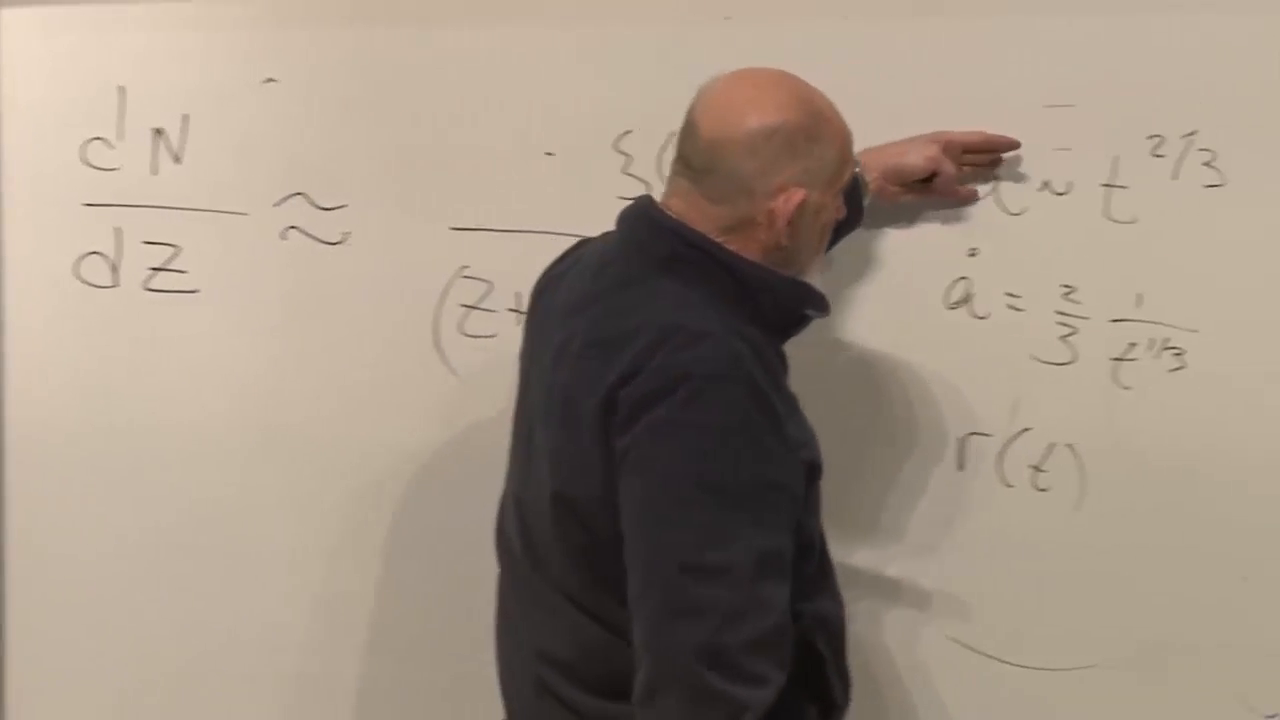
\includegraphics[width=0.84\textwidth]{lecture_06_figure_05.png}
\caption{黑板上\(dN/dz\)與模型函數的關係。左側以及右側的\(a\sim t^{2/3}\)、\(\dot a\)和\(r(t)\)都可見，但講師遮住分母的一部分；方程~\eqref{eq:c06-dndz}已在前文獨立推導。}
\label{fig:c06-dndz-board}
\lectureframe{01:22:24.114}
\end{figure}

選定模型之前，還沒有可進一步計算的內容。指定\(a(t)\)便能決定\(\dot a(t)\)，方程~\eqref{eq:c06-null-ray}決定\(r(t)\)，而方程~\eqref{eq:c06-redshift}則能讓所有量都以\(z\)表示。不同的狀態方程會產生不同的函數\(dN/dz\)和\(F(z)\)。這正是觀測能夠區分不同模型的原因。

\section{從試探參數到最佳擬合}

程序很直接：
\begin{equation}
(\Omega_r,\Omega_m,\Omega_\Lambda,\Omega_k)
\longrightarrow
a(t)
\longrightarrow
\left\{F(z),\frac{dN}{dz}\right\}.
\label{eq:c06-fit-pipeline}
\end{equation}
選定當下參數，求解弗里德曼方程，沿徑向傳播光線，計算亮度與源計數隨紅移的變化，再將曲線與資料比較。若比較結果不符，就排除該組參數。兩種觀測量合在一起，可約束膨脹歷史和空間幾何。

\begin{figure}[htbp]
\centering
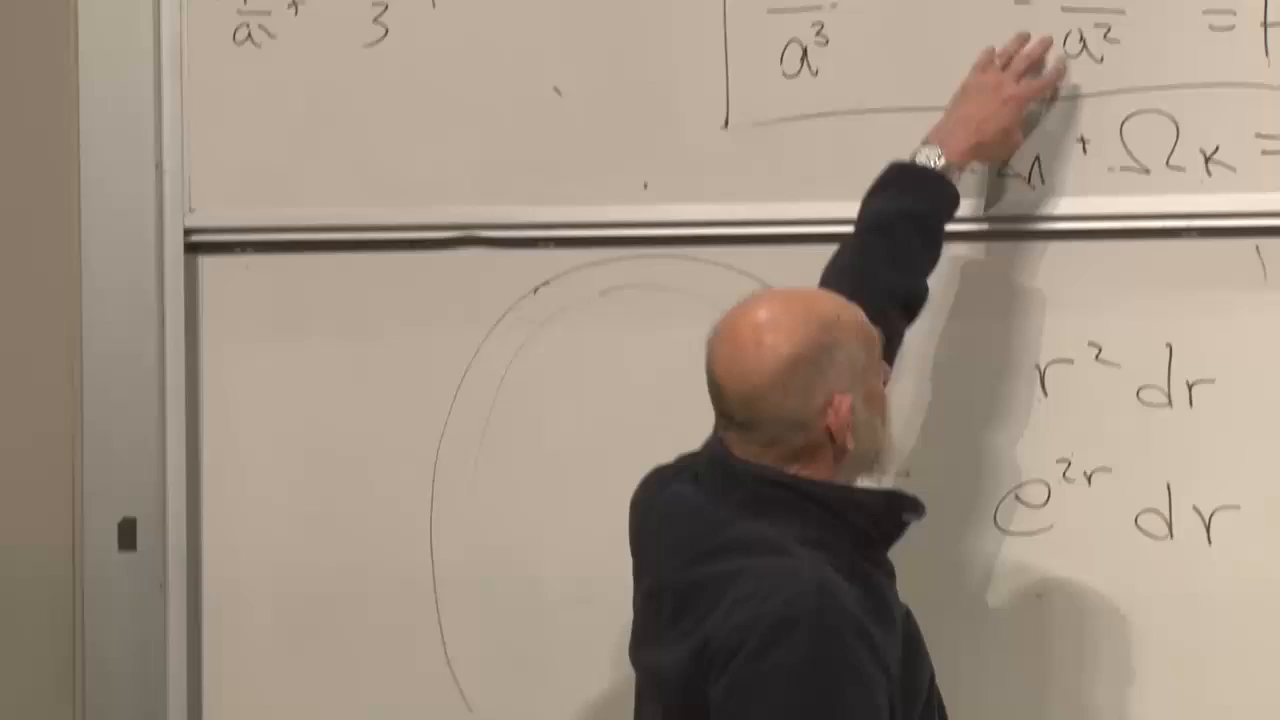
\includegraphics[width=0.84\textwidth]{lecture_06_figure_06.png}
\caption{上方黑板顯示舊的物質加曲率模型，下方黑板則顯示平坦與雙曲殼層因子\(r^2dr\)和\(e^{2r}dr\)。弗里德曼方程有部分內容被遮住，因此這個畫面僅作為輔助證據，並非方程的來源。}
\label{fig:c06-old-model-board}
\lectureframe{01:24:27.863}
\end{figure}

舊模型
\begin{equation}
H^2=\frac{C_m}{a^3}-\frac{k}{a^2},
\qquad k=-1,
\end{equation}
無法通過亮度－紅移關係和源計數兩項檢驗。在相關紅移範圍內，超新星是最實用的標準燭光。本講得到的成功參數組為
\begin{equation}
\boxed{
\Omega_r\simeq0,\qquad
\Omega_m\simeq0.3,\qquad
\Omega_\Lambda\simeq0.7,\qquad
\Omega_k\simeq0
}.
\label{eq:c06-best-fit}
\end{equation}
此處的物質包含發光物質和暗物質。這些數值反映本講當時的擬合結果；值得保留的是擬合方法，以及宇宙需要一個占主導地位且不會稀釋的成分，而不是最後印出的那一位小數。

\subsection{關於測量值與擬合值的問題}

\begin{classroomqa}
\audiencequestion{討論舊的開放宇宙模型時，就已經假設\(\Lambda\)了嗎？}
\lecturerresponse{沒有。第一部分刻意以\(\Lambda=0\)重建舊模型。方程~\eqref{eq:c06-best-fit}中的數值描述的是後來的現代擬合。舊的候選模型並未被悄悄修改，而是接受\(F(z)\)和\(dN/dz\)的檢驗，結果未能通過。 \lecturetimestamp{01:26:45--01:27:07}}
\end{classroomqa}

\begin{classroomqa}
\audiencequestion{如果真空能不像局部物質那樣能直接測量，\(\Omega_\Lambda\)是如何得到的？}
\lecturerresponse{從一組組試探參數開始。每組參數都定義一個弗里德曼解，因此也定義出預測函數\(F(z)\)和\(dN/dz\)。將預測與觀測比較，排除擬合不佳的組合，再保留參數空間中擬合最好的區域。數值\(0.7\)是由擬合推論而得，並非直接從真空能測量儀讀出。 \lecturetimestamp{01:27:08--01:29:59; 01:31:57--01:33:40}}
\end{classroomqa}

\begin{classroomqa}
\audiencequestion{現今的尺度因子 \(a_0\)從何而來？}
\lecturerresponse{\(a\)的正規化有一部分是約定俗成的；不過，若模型已完整建立並與 \(H_0\) 相聯繫，那麼在 \(k\ne0\) 時，模型便會給出現今的物理曲率尺度。模型一旦符合紅移觀測量，其函數 \(a(t)\) 就會標示出現今所處的位置及其對應尺度。\lecturetimestamp{01:29:59--01:30:42}}
\end{classroomqa}

\begin{classroomqa}
\audiencequestion{回望數十億年前的宇宙，會不會使以現今參數為基礎的擬合產生偏差？}
\lecturerresponse{回望過去並不是偏差；它本身就是訊號。將現今參數代入弗里德曼方程，方程便會將它們演化成完整的 \(a(t)\)。預測的光錐已納入這項事實：在較小的 \(a\) 時，物質的影響較大；回溯到足夠早的時期，則由輻射主導。忽略這種演化的模型將無法符合觀測資料。\lecturetimestamp{01:30:43--01:31:55}}
\end{classroomqa}

\begin{classroomqa}
\audiencequestion{哪些現今的物理量相對容易直接測量？}
\lecturerresponse{輻射密度可以測量，但在現今可忽略不計。哈伯率可由距離與紅移的關係測得。總物質密度則由引力效應推得，包含發光物質與暗物質；再除以臨界尺度 \(3H_0^2/(8\pi G)\)，即可得到 \(\Omega_m\)。晚期宇宙尚待決定的自由度，主要是真空能與曲率。\lecturetimestamp{01:33:40--01:35:32}}
\end{classroomqa}

\begin{classroomqa}
\audiencequestion{如果 \(\Omega_\Lambda\) 和 \(\Omega_k\) 都未知，為什麼在固定 \(\Omega_m\) 之後，晚期模型試算只剩一個獨立參數？}
\lecturerresponse{因為方程 ~\eqref{eq:c06-sum-rule} 施加了一項約束。當 \(\Omega_r\) 可忽略，且 \(\Omega_m\) 已測得時，選定一個試算值 \(\Omega_\Lambda\)，就會決定剩餘的 \(\Omega_k=1-\Omega_m-\Omega_\Lambda\)。同一個一維參數族也可以用曲率來表示。例如，當 \(\Omega_m=0.3\) 時，取 \(\Omega_\Lambda=0.4\) 和 \(\Omega_k=0.3\) 作為試算值是可行的；這組參數遭到排除，只是因為預測曲線的擬合效果不佳，並非求和規則禁止這種組合。\lecturetimestamp{01:35:33--01:39:09}}
\end{classroomqa}

\begin{classroomqa}
\audiencequestion{\(k\)怎麼會只有 \(+1,0,-1\) 這幾個離散值，而 \(\Omega_k\) 卻連續變化？量綱也正確嗎？}
\lecturerresponse{離散的 \(k\) 只記錄符號與正規化後的幾何性質。連續變化的曲率半徑則由 \(a_0\) 表示，因此 \(-k/(a_0^2H_0^2)\) 可以連續取值。在 \(c=1\) 單位制中，逆長度與逆時間的量綱相同；恢復慣用單位後，所需的 \(c\) 次方就會補上。\lecturetimestamp{01:39:10--01:40:07}}
\end{classroomqa}

\begin{classroomqa}
\audiencequestion{計數方法是否假設了均勻性與各向同性，儘管星系族群會隨時間演化？}
\lecturerresponse{這個方法假設在足夠大的空間切片上具有均勻性與各向同性；比較同一紅移下不同方向的觀測結果，可以檢驗這些對稱性。源的演化則是另一個問題：不同時期的族群不必完全相同，因此實際分析會將選擇效應與演化納入模型，而不會假設數密度永遠固定。這個簡單推導先單獨呈現幾何因子，再加入這些修正。\lecturetimestamp{01:40:08--01:41:08}}
\end{classroomqa}

\section{密度參數隨時間演化}

方程~\eqref{eq:c06-budget}在每個時刻都成立，但方程~\eqref{eq:c06-omegas}中的\(\Omega\)是在現今定義的。它們隨時間變化的對應量之所以會改變，是因為四項對\(a\)的依賴次方各不相同。在遙遠的過去，
\begin{equation}
\Omega_r(t)\longrightarrow1.
\end{equation}
輻射稀釋得較快，因此物質的相對占比上升，逐漸取得主導地位。之後，物質本身也會稀釋，而\(\Lambda\)保持不變，因此在遙遠的未來，
\begin{equation}
\Omega_\Lambda(t)\longrightarrow1.
\end{equation}
所以，物質占比起初很小，在物質主導時期接近於一，等真空能取得主導地位後又再次下降。若曲率不為零，最終也會逐漸不及正的常數\(\Lambda\)重要。

\begin{classroomqa}
\audiencequestion{現今曲率占比很小，是否表示宇宙會隨膨脹而變得越來越平坦？}
\lecturerresponse{宇宙的物理曲率尺度會隨著\(a\)增大；相對於正的宇宙常數，曲率項\(a^{-2}\)的影響也會越來越小。這就是「\emph{尺度愈大，空間愈平坦}」這句話的意思。這不會改變離散的拓撲標籤\(k\)；它描述的是局部曲率，以及曲率在動力學中的相對重要性逐漸降低。\lecturetimestamp{01:47:13--01:47:42}}
\end{classroomqa}

\begin{classroomqa}
\audiencequestion{擬合模型是否出現無法解釋的系統性殘差？這項說法的精確度有多高？}
\lecturerresponse{講座指出，在當時的精度下，這個架構沒有已知的系統性失效，並將之稱為精度約在百分之一量級的宇宙學，而非精確到千分之一或萬分之一。這是對當時情況的描述，不應視為永遠適用的現今誤差範圍。\lecturetimestamp{01:45:40--01:46:19}}
\end{classroomqa}

\begin{classroomqa}
\audiencequestion{除了超新星亮度和計數之外，能否透過直接三角測量來檢驗空間曲率？}
\lecturerresponse{可以。宇宙微波背景的角向分布提供一個標準物理尺度，因此可以構成一個尺度極大的宇宙三角形。僅憑超新星資料，無法得出講座所述完整的百分之一量級曲率精度；結合微波背景幾何後，這項檢驗會更加精確。這是下一講的主題。\lecturetimestamp{01:46:19--01:47:12}}
\end{classroomqa}

\section{帶走的核心觀念}

核心觀念不是列出四個數字，而是一種方法。一組宇宙學參數會決定 \(a(t)\)；度規接著預測光的傳播、光源亮度與光源計數。預測與觀測是否相符，既檢驗所選的參數，也檢驗將這些參數聯繫起來的弗里德曼架構。任意一組參數未必都能符合觀測。

舊的「只有發光物質且具有負曲率」模型失敗了。暗物質補足了引力物質的組成，但僅靠暗物質，仍無法補足舊弗里德曼模型的能量預算。講座當時成功的擬合需要大約
\begin{equation}
\Omega_m\simeq0.3,
\qquad
\Omega_\Lambda\simeq0.7,
\qquad
\Omega_k\simeq0,
\end{equation}
而其曲率精度很大程度上取決於微波背景。這個模型之所以可信，是因為多項彼此獨立的觀測都經由同一套動力學理論描述，並匯聚到參數空間的同一區域。